% !TeX encoding = UTF-8
\chapter{Task 2: Deep Learning}\label{chap:task2}

\section{Models}
We implement the three models in PyTorch \cite{pytorch}. Each takes the same 59 standardized features and outputs one logit; the sigmoid of the logit is the score for DDoS.

\begin{table}[htb]
\centering
\caption{Architectures of the neural networks ($f=59$ input features).}\label{tab:arch}
\begin{tabular}{lp{12cm}}
\toprule
Model & Architecture \\
\midrule
MLP & $f \to 128 \to 64 \to 1$, ReLU, dropout 0.2 \\
LSTM \cite{lstm} & the features are read as a sequence of $f$ steps with one value each; \texttt{LSTM(input\_size=1, hidden\_size=32, batch\_first=True)}; the last hidden state feeds a linear layer ($32 \to 1$) \\
1D-CNN & the features form a one-channel signal of length $f$; Conv1d($1 \to 32$, $k=3$) + ReLU + max-pool 2, Conv1d($32 \to 64$, $k=3$) + ReLU, global max-pool, linear ($64 \to 1$) \\
\bottomrule
\end{tabular}
\end{table}

Flow features have no natural order, so the sequence and convolution models treat the feature vector as a pseudo-sequence. We use them because the task asks for them; the data itself is not sequential.

\section{Training}
All networks minimize the binary cross-entropy with the Adam optimizer \cite{adam}, with batch size 1024 and a shuffling generator seeded with 42. After every epoch we compute the validation loss; training stops when it has not improved for \emph{patience} epochs, and the weights of the best epoch are restored. Table~\ref{tab:dl-settings} lists the settings.

\begin{table}[htb]
\centering
\caption{Training settings and outcome of the final run (LR = learning rate, Clip = gradient-norm clipping, ep. = epoch; best epoch = lowest validation loss).}\label{tab:dl-settings}
\small\setlength{\tabcolsep}{4pt}
\begin{tabular}{lrrrrrrr}
\toprule
Model & LR & Patience & Max ep. & Clip & Stopped & Best ep. & Best val.\ loss \\
\midrule
MLP & $10^{-3}$ & 3 & 40 & -- & 32 & 29 & 0.00167 \\
LSTM & $5\cdot10^{-4}$ & 7 & 40 & 1.0 & 38 & 31 & 0.00529 \\
1D-CNN & $10^{-3}$ & 3 & 30 & -- & 25 & 22 & 0.00360 \\
\bottomrule
\end{tabular}
\end{table}

\paragraph{Epoch limits.} With a limit of 15 epochs no network had stopped early, so they may have been under-trained. We raised the limits; with a limit of 30, the best validation epochs were 29 for the MLP and 22 for the CNN. Because the MLP's best epoch sat at the limit, we raised its limit to 40, and it then stops by itself at epoch 32 with the same best epoch. The first choice of the limits was made by comparing test metrics, which is a limitation (limitation 4 in \cref{chap:discussion}).

\paragraph{LSTM instability.} With the shared settings (learning rate $10^{-3}$, patience 3, no clipping) the LSTM trained unstably: the training loss spiked after a few epochs, probably from exploding gradients over the 59-step sequence on heavy-tailed inputs. This gave an F1 of 0.9943 (101 false positives, 118 false negatives) after 15 epochs. We therefore added gradient-norm clipping at 1.0 \cite{pascanu2013clip} and gave the LSTM its own learning rate and patience. We chose these by the lowest \emph{validation} loss over three configurations: learning rate $5\cdot10^{-4}$ with patience 7 and a limit of 40 epochs reached 0.00529, ahead of $5\cdot10^{-4}$ with patience 5 and a limit of 30 (0.00567, which hit its limit) and $3\cdot10^{-4}$ with patience 5 and a limit of 40 (0.00720). With the chosen settings the LSTM improves on every test metric (F1 0.9943 $\to$ 0.9992). The validation loss still oscillates (Figure~\ref{fig:history}), so clipping reduces the instability but does not remove it.

\begin{figure}[htb]
\centering
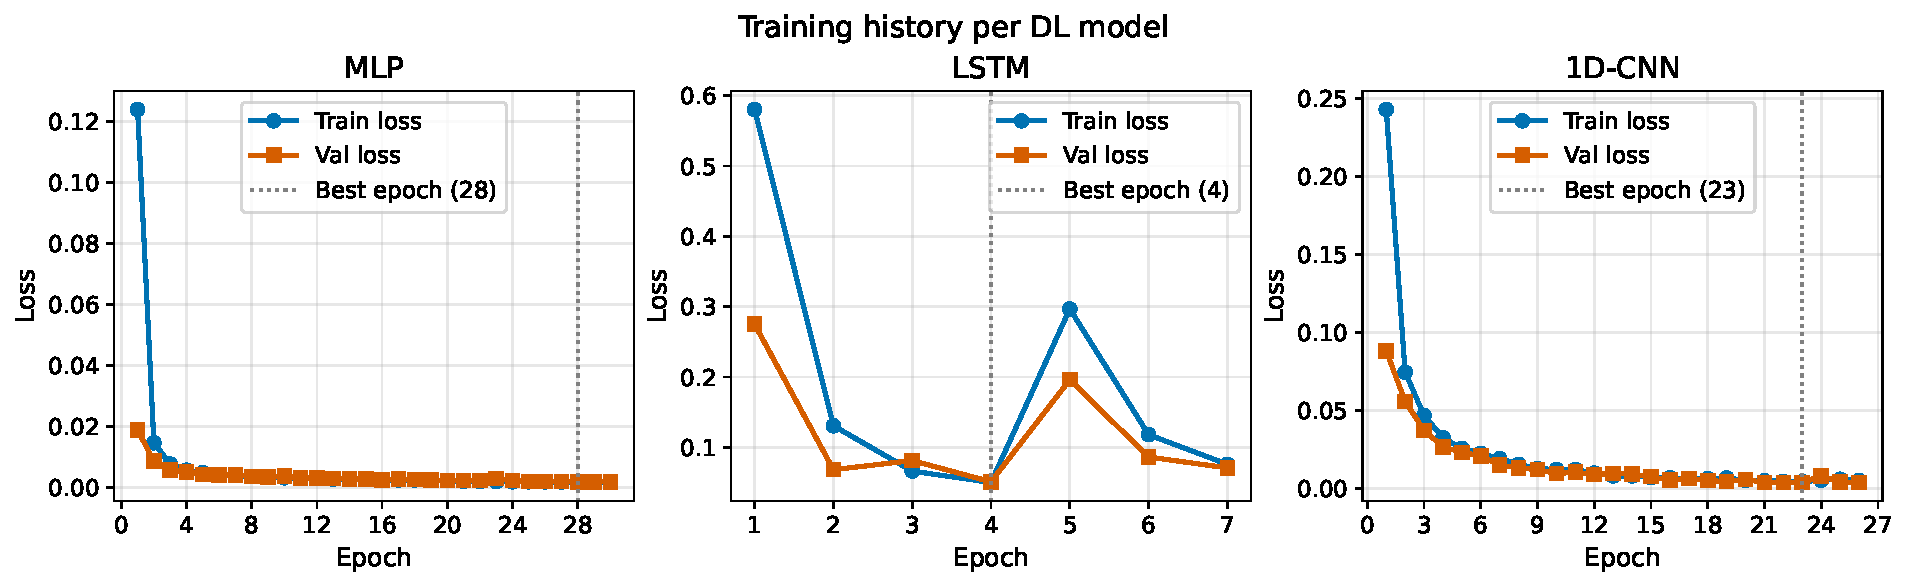
\includegraphics[width=\textwidth]{dl_history_grid.pdf}
\caption{Training and validation loss (log scale) of the three networks. The dotted line marks the epoch whose weights are restored. The LSTM's validation loss is much noisier than that of the MLP and the CNN.}\label{fig:history}
\end{figure}
